Ein Wagen wird auf einer geraden Bahn angestossen und rollt eine schiefe Ebene hinauf. Eine Stroboskopaufnahme zeigt ihn einmal pro Sekunde, von $t = 0$ bis $t = \SI{5}{\second}$. Über jedem Punkt steht die Zeit; bei zwei Punkten liegen die Bilder von zwei Zeitpunkten genau übereinander.
\begin{center}
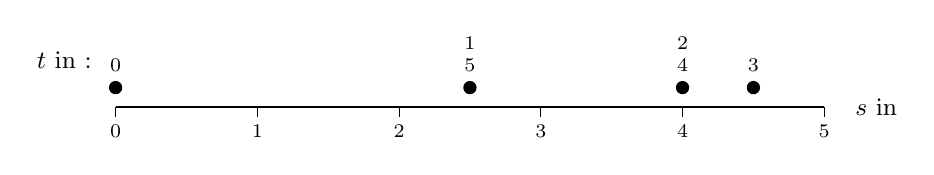
\begin{tikzpicture}[x=1.8cm, y=1cm]
 \draw[thick] (0,0) -- (5,0);
 \foreach \sk in {0,...,5} \draw (\sk,0) -- (\sk,-0.12);
 \foreach \sk in {0,1,...,5} \node[below, font=\scriptsize] at (\sk,-0.1) {$\sk$};
 \fill[black] (0,0.25) circle (2.4pt);
 \fill[black] (2.5,0.25) circle (2.4pt);
 \fill[black] (4,0.25) circle (2.4pt);
 \fill[black] (4.5,0.25) circle (2.4pt);
 \node[above, font=\scriptsize, align=center] at (0,0.33) {$0$};
 \node[above, font=\scriptsize, align=center] at (2.5,0.33) {$1$\\$5$};
 \node[above, font=\scriptsize, align=center] at (4,0.33) {$2$\\$4$};
 \node[above, font=\scriptsize, align=center] at (4.5,0.33) {$3$};
 \node[right, font=\small] at (5.15,0) {$s$ in \si{\meter}};
 \node[left, font=\small] at (-0.1,0.6) {$t$ in \si{\second}:};
\end{tikzpicture}
\end{center}
\begin{abcliste}
\abc \DuSie{Skizziere}{Skizzieren Sie} das $s(t)$-Diagramm.
\abc Wann und wo kehrt der Wagen um? Wie gross ist seine Geschwindigkeit in diesem Moment?
\abc \DuSie{Zeige}{Zeigen Sie}, dass die Bewegung gleichmässig beschleunigt ist, und \DuSie{bestimme}{bestimmen Sie} die Beschleunigung (mit Vorzeichen).
\end{abcliste}
